% Chapter 3

\chapter{ارائه معماری دوقلوی دیجیتال چندعاملی}


\section{مقدمه}

دوقلوی دیجیتال چندعاملی\LTRfootnote{Multi-Agent Digital Twin} به عنوان یک الگوی دیجیتال فراگیر برای شبیه‌سازی و مدیریت سیستم‌های پیچیده در حوزه‌های مختلف، از جمله تولید، حمل‌ونقل و بهداشت، تعریف می‌شود. این مدل به سازمان‌ها امکان می‌دهد تا با ایجاد یک نسخه مجازی از سیستم‌های فیزیکی خود، اطلاعات و داده‌های مربوط به عملکرد آن‌ها را به‌طور دقیق رصد و تحلیل کنند.

دوقلوی دیجیتال از اجزای مختلفی تشکیل شده است که هر کدام به‌واسطه جمع‌آوری داده‌ها، پردازش اطلاعات و تجزیه و تحلیل نتایج به کارایی این سیستم کمک می‌کند. به کارگیری فناوری‌های هوش مصنوعی، یادگیری ماشین و اینترنت اشیا در دوقلوی دیجیتال چندعاملی، می‌تواند به بهبود تصمیم‌گیری و پیش‌بینی‌های دقیق‌تر، کمک کند. در این راستا، بخش‌های مختلف دوقلوی دیجیتال شامل حسگرها، گره‌های پردازش و ابزارهای تحلیلی به‌طور هماهنگ و یکپارچه با هم ارتباط برقرار می‌کنند تا بتوانند نتایج علمی و قابل انجامی را به ثمر رسانند. در اینجا نیز یک نمونه از معماری دوقلوی دیجیتال چندعاملی مورد بررسی قرار گرفته است.
\cite{b15}

\section{معماری ابر-مه-لبه}
معماری ابر-مه-لبه\LTRfootnote{Cloud-Fog-Edge}
یک چارچوب چندلایه است که برای مدیریت و پردازش داده‌های دوقلوی دیجیتال طراحی شده است. همانطور که در تصویر \ref{fig:layers_arch} مشاهده‌ می‌شود، این معماری شامل سه لایه اصلی است. این  سه لایه دربردارنده لایه ابر، لایه مه و لایه لبه است که هر کدام نقش مهمی در تسهیل عملیات و پردازش داده‌ها دارند.
\subsection{لایه ابر}

لایه ابر به‌عنوان هسته مرکزی این معماری عمل می‌کند و شامل چندین عملکرد کلیدی است:
\begin{itemize}
	\item ذخیره‌سازی داده‌ها\LTRfootnote{Data Storage}:
	این لایه امکان ذخیره‌سازی مقیاس‌پذیر و امن داده‌های جمع‌آوری‌شده را فراهم می‌کند. داده‌های بزرگ که از دستگاه‌ها و حسگرها دریافت می‌شوند، در این لایه به‌صورت متمرکز نگهداری می‌شوند.
	
	\item 
	تحلیل و پردازش\LTRfootnote{Data Analytics}: 
	لایه ابر از ابزارهای تحلیلی پیشرفته و الگوریتم‌های یادگیری ماشین برای تجزیه و تحلیل داده‌ها استفاده می‌کند. این ابزارها می‌توانند به شناسایی الگوها، روندها و پیش‌بینی‌های مؤثر کمک کنند که نتیجه‌ی آن بهبود تصمیم‌گیری‌های سازمانی در راستای انجام عملیات‌های پیچیده و بهبود کارایی است.
	
	\item
	شبیه‌سازی\LTRfootnote{Simulation}:
	 این لایه قابلیت شبیه‌سازی فرآیندها و ارزیابی آثار تغییرات مختلف را فراهم می‌کند. این توانایی به سازمان‌ها اجازه می‌دهد تا حالت‌های مختلف را بررسی کرده و به شبیه‌سازی رفتار سیستم در شرایط متفاوت بپردازند.
	
\end{itemize}

\subsection{لایه مه}

لایه مه به‌عنوان واسط میان لایه ابر و لایه لبه عمل می‌کند و هدف آن پردازش محلی و کاهش تأخیر در عملیات‌ها است:
\begin{itemize}
	\item 
	
گره‌های ثابت مه\LTRfootnote{Static Fog Nodes}:
	این نودها در مکان‌های خاص مانند ایستگاه‌ها یا مراکز داده محلی قرار دارند و وظیفه پردازش داده‌های محلی و انجام تحلیل‌های سریع را بر عهده دارند. این گره‌ها، زمان واکنش‌ را بهبود می‌بخشند و برای پردازش‌های محلی بسیار مفید هستند.
	
	\item 
	
نودهای متحرک مه\LTRfootnote{Dynamic Fog Nodes}:
	این نودها به سیستم‌های متحرک مانند خودروها، پهپادها یا ربات‌ها متصل می‌شوند و می‌توانند داده‌ها را از مکان‌های مختلف جمع‌آوری کنند. این گره‌ها به مدیریت داده‌ها در مناطقی با دسترسی محدود به اینترنت و مناطق سخت‌ گذر که به راحتی در دسترس انسان نیست، کمک می‌کنند.
\end{itemize}

\subsection{لایه لبه}

لایه لبه شامل دستگاه‌ها و حسگر‌هایی\LTRfootnote{Sensors} است که به‌طور مستقیم اطلاعات را از محیط جمع‌آوری می‌کنند. این لایه به‌عنوان چشم و گوش سامانه عمل می‌کند و با لایه مه در ارتباط است. این لایه شامل بخش‌های زیر است:
\begin{itemize}
\item 
حسگرها و عملگرها: این دستگاه‌ها، داده‌های ضروری را از محیط جمع‌آوری می‌کنند. این اطلاعات می‌تواند شامل دما، رطوبت، سرعت و دیگر مولفه‌های مرتبط و مورد نیاز باشد. این بخش همچنین شامل دستگاه‌های عملگر مانند بازو‌های مکانیکی و الکترونیکی جهت انجام دستور دریافت شده است.
\item 
تحلیل محلی: پردازش اولیه داده‌ها در لایه لبه انجام می‌شود تا فقط داده‌های مورد نیاز به لایه‌های بالاتر ارسال شوند. این کار نه‌تنها باعث صرفه‌جویی در پهنای باند می‌شود بلکه زمان واکنش به رخدادها نیز کاهش می‌یابد.

\item 
ارتباطات با لایه مه: دستگاه‌های لبه به‌طور مستقیم با خدمات لایه مه ارتباط برقرار می‌کنند و اطلاعات و دستورات را به‌صورت منطقه‌ای، ارسال و دریافت می‌کنند. نوع ارتباط در این  لایه می‌تواند بنا به شرایط محیط، متفاوت باشد. انواع ارتباط‌های سیمی و بی‌سیم، راه‌ نزدیک و راه دور، می‌تواند بخشی از این لایه باشد.

\end{itemize}

\begin{figure}[htb]
	\centering
	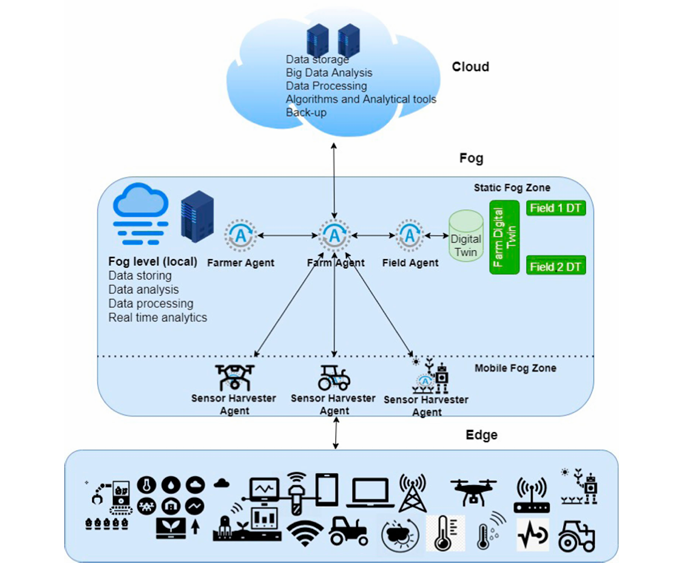
\includegraphics[width=1\textwidth]{./Images/arch.png}
	\caption{معماری ابر-مه-لبه \cite{b15}}
	\label{fig:layers_arch}
\end{figure}

\section{استفاده از دوقلوی دیجیتال در معماری پیشنهادی}
معماری دوقلوی دیجیتال یکی از بخش‌های مرکزی معماری ارائه‌شده به حساب می‌آید. این دوقلوی دیجیتال زمینه اصلی فعالیت‌های عامل‌ها را فراهم می‌کند و با آن‌ها ارتباط برقرار کرده و پردازش‌های لازم جهت ایجاد دوقلوی دیجیتال را انجام می‌دهد.
داده‌های خام سنسور از دستگاه‌های لبه‌\LTRfootnote{Edge devices} که در محیط مستقر شده‌اند توسط نوع خاصی از عامل به نام "برداشت‌کننده سنسور" جمع‌آوری می‌شود.
منابع داده خارجی نیز مانند داده‌های هواشناسی، ماهواره‌ای یا حتی داده‌های مالی این داده‌ها را تکمیل می‌کنند و همراه با خدمات تحلیل داده مبتنی بر ابر \LTRfootnote{Cloud-based Data Analytics} برای ارائه بینش‌ها و نتایجی که عامل‌ها می‌توانند انجام دهند،استفاده می‌شوند.
برخی از این بینش‌ها و نتایج به بهبود دقت دوقلوی دیجیتال کمک می‌کنند و تصمیم‌گیری را ساده‌تر می‌کنند. همچنین با استفاده از پردازش‌های ابر، می‌توان برنامه‌های دقیقی برای کاربرد‌های گوناگون ارائه گردد و برای اجرای آن، برنامه ریزی شود.
مدل دوقلوی دیجیتال در این معماری به کاربران کمک می‌کند اطلاعاتی در مورد محیط و رفتار کلی سیستم به دست آورند و پیش‌بینی‌ها، مراحل، اطلاعات و گزارش‌هایی را دریافت کنند به طوری که قابل درک‌تر برای انسان و ماشین باشد.


\section{ساختار معماری دوقلوی دیجیتال}

معماری دوقلوی دیجیتال به‌عنوان یک سیستم پیشرفته برای مدیریت و بهینه‌سازی فرآیندها در حوزه‌های مختلف، طراحی‌ شده است. این معماری شامل چهار لایه کلیدی است که هر یک نقش مهمی در کارکرد صحیح و بهینه‌سازی عملکرد دوقلوی دیجیتال و عامل‌ها ایفا می‌کنند. در تصویر \ref{fig:dt_layers} می‌توان لایه‌های این معماری را مشاهده کرد که در ادامه به توضیح لایه‌ها پرداخته می‌شود.

\begin{figure}[htb]
	\centering
	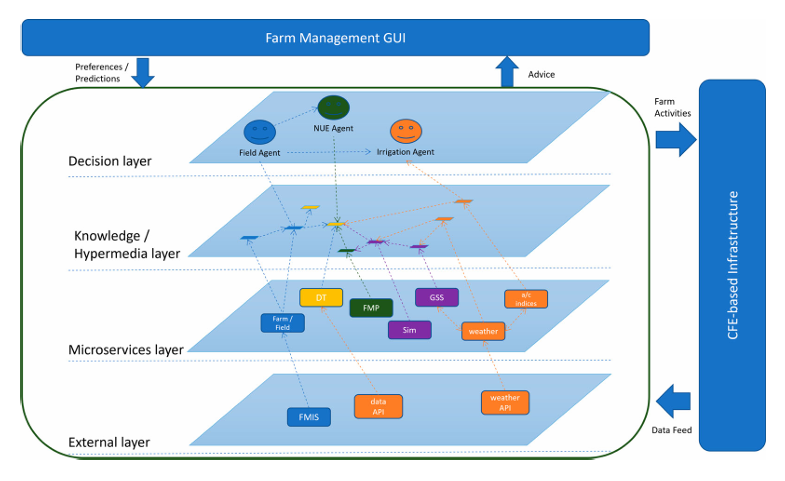
\includegraphics[width=1\textwidth]{./Images/dt.png}
	\caption{معماری لایه‌ای دوقلوی دیجیتال \cite{b15}}
	\label{fig:dt_layers}
\end{figure}

\subsection {لایه خارجی}
لایه اول، لایه خارجی است که زیرساخت اساسی دوقلوی دیجیتال را تشکیل می‌دهد و شامل منابع کلیدی نظیر خدمات داده،تهیه اطلاعات و خدمات پیش‌بینی است. این لایه دسترسی به سیستم‌های اطلاعاتی را فراهم می‌کند که می‌تواند داده‌های لازم را جمع‌آوری و تحلیل کند. داده‌های به دست آمده از حسگرها و فناوری‌های اینترنت اشیاء در این لایه جمع‌آوری می‌شوند تا اطلاعات مورد نیاز برای تصمیم‌گیری و نتیجه‌گیری به گونه‌ای موثر فراهم شود.
\subsection {لایه میکروسرویس‌ها}
لایه دوم، لایه میکروسرویس‌ها\LTRfootnote{Microservices} است که مسئول تبدیل خدمات ارائه‌شده در لایه خارجی به فرمت‌های استاندارد بر اساس هستی‌شناسی\LTRfootnote{Ontology} مورد نیاز تعریف ‌شده است. در این لایه، خدمات داخلی تخصصی برای دوقلوی دیجیتال طراحی و ارائه می‌شوند. این خدمات می‌توانند شامل برنامه‌ریزی و مدیریت داده‌ها باشند که نقاط تصمیم‌گیری را برای مراحل مختلف فرآیندها ثبت کنند. همچنین، این لایه می‌تواند به شبیه‌سازی رفتارهای واقعی یا مجازی در طول زمان بپردازد و از این طریق زمینه‌ای برای اتخاذ تصمیمات دقیق‌تری فراهم کند.
\subsection{لایه دانش/ابررسانه}
لایه سوم، لایه دانش یا ابررسانه\LTRfootnote{Hypermedia} است که ارتباط بین داده‌ها و محتوای دانش را تسهیل می‌کند. این لایه شامل منابعی است که به‌صورت داده‌های متصل و در ارتباط با هم، تعریف‌شده‌اند و بر اساس هستی‌شناسی‌های مشخص سازمان‌دهی و دسته‌بندی شده‌اند. ساختار این اطلاعات به‌گونه‌ای طراحی شده که به آسانی قابل مدیریت و تحلیل باشد. به‌این‌ترتیب، این لایه به‌عنوان یک گراف دانش عمل کرده و تمام اطلاعات موجود را یکپارچه می‌کند و امکان تبدیل داده‌ها به دانش قابل استفاده را فراهم می‌سازد.
\subsection{لایه تصمیم‌گیری}
لایه چهارم، لایه تصمیم‌گیری است که اجرا‌کننده کلیه فعالیت‌های مربوط به تصمیم‌سازی در دوقلوی دیجیتال است. این لایه شامل طراحی عامل‌های خاصی است که وظیفه نظارت و تحلیل داده‌ها را برعهده دارند. این عامل‌ها می‌توانند با استفاده از اطلاعات و ترجیحات کاربر، به نظارت بر عملیات‌ها پرداخته و تصمیمات مناسب را در زمان درست اتخاذ کنند. همچنین، این لایه استانداردهایی را برای تعامل با سایر عامل‌ها فراهم می‌کند و از این طریق امکان تصمیم‌گیری‌های هوشمند و خودکار نیز بوجود می‌آید.

\section{جمع‌بندی}

این معماری به‌گونه‌ای طراحی شده که بتواند به‌راحتی برای انجام وظایف جدید گسترش یابد و با فناوری‌های جدید و الزامات متنوع سازگاری یابد. ایجاد توصیفات وظیفه به‌صورت قابل انعطاف و طراحی عامل‌های جدید برای انواع وظایف، این سیستم را قادر می‌سازد که هر زمان که نیاز باشد کارایی خود را افزایش دهد.

وجود عامل‌های مختلف و ارتباط آن‌ها با یکدیگر در این معماری، به انعطاف‌پذیری، مقیاس‌پذیری و کارایی دوقلو‌های دیجیتال کمک چشم‌گیری می‌کند به طوری که در صورت ایجاد نیازمندی جدید در سامانه،‌ می‌توان با اضافه کردن عامل مربوط و مناسب برای آن نیازمندی، به صورت کامل و صحیح آن را پاسخ داد.

در نهایت، استفاده از داده‌های ساختاریافته و مرتبط در دوقلوی دیجیتال تبادل دانش و اطلاعات را ساده‌تر کرده و امکان تعامل میان حوزه‌های مختلف را فراهم می‌کند. با یکپارچه‌سازی منابع داده‌ای متنوع، این معماری می‌تواند تصمیم‌گیری‌های مؤثر و دقیقی را ارائه دهد که به بهبود فرآیندها و استفاده بهینه از منابع کمک می‌کند. به این ترتیب، معماری دوقلوی دیجیتال و چندعاملی، به‌عنوان ابزار نوآورانه‌ای در حوزه‌های مختلف، این امکان را فراهم می‌کند که عملکردها بهینه شوند و نتایج بهتری به‌دست آید.